%
% Author: Kian Ho <hui.kian.ho@gmail.com>
%
% Description:
%
%   Seminar slides for introducing COMBINE, who we are, our aims, and events.
%   You could also print these slides and pin them up at conferences as a quick
%   alternative to a proper flyer or poster.
%
% Compilation:
%
%   Latex, beamer, and 'scons' need to be installed, which is easily done using
%   modern Linux distributions such as Ubuntu. SCons automatically handles the
%   latex dependencies during compilation.
%
%   Run 'make' to compile the slides, this in-turn calls 'scons', but you need
%   to ensure that the necessary latex packages are installed. You can do this
%   by searching for the packages named in the '\usepackage{...}' commands in
%   the preamble.
%
%   Run 'make clean' to delete all the latex-generated files prior to a fresh
%   re-compilation.
%

\documentclass[svgnames]{beamer}
    \beamertemplatenavigationsymbolsempty
    \usetheme{Singapore}

    \makeatletter

    % Change default item bullets from circles to the default triangles. 
    \setbeamertemplate{itemize items}{\raise1.25pt\hbox{\scriptsize$\blacktriangleright$}}

    % Simple footer for each slide showing only the slide number / total slides.
    \setbeamertemplate{footline}
    {
        \begin{minipage}[c]{0.97\paperwidth}
            \raggedleft
            \usebeamerfont{date in head/foot}\usebeamercolor[fg]{title}\insertframenumber{} / \inserttotalframenumber
        \end{minipage}
        \vspace{1.5ex}
    }

    \makeatother

    \usepackage{varwidth}
    \usepackage{xcolor}
    \usepackage{graphicx}
    \usepackage{hyperref}
    \usepackage{verbatim}
    \usepackage{varwidth}
    \usepackage{microtype}

    \newcommand{\beamerpurple}[1]{{\usebeamercolor[fg]{title}#1}}
\begin{document}

\begin{frame}
    \vfill
    \begin{minipage}[c]{\linewidth}
        \centering
        \hfill
        \begin{minipage}[c]{0.45\linewidth}
            \centering
            
\includegraphics[width=\linewidth]{./images/COMBINE-logo.png}
        \end{minipage}
        \begin{minipage}[c]{0.45\linewidth}
            \centering
            
\includegraphics[height=20mm]{./images/RSGAU-logo.png}
        \end{minipage}
        \hfill
    \end{minipage}
    \vfill
    \beamerpurple{COMBINE} is a student-run Australian organisation for researchers in
    \textbf{computational biology}, \textbf{bioinformatics}, and related
    fields.\\[2ex]
    We aim to bring together students and early-career
    researchers from the computational and life sciences for networking,
    collaboration, and professional development.\\[1ex]
    \begin{itemize}
        \item we run seminars, workshops, symposiums, and social events.
        \item we are the official
        \href{http://www.iscb.org/}{\beamerpurple{ISCB}} Regional Student Group for
        Australia.
    \end{itemize}
    \vfill
\end{frame}

\begin{frame}{Previous Events}
    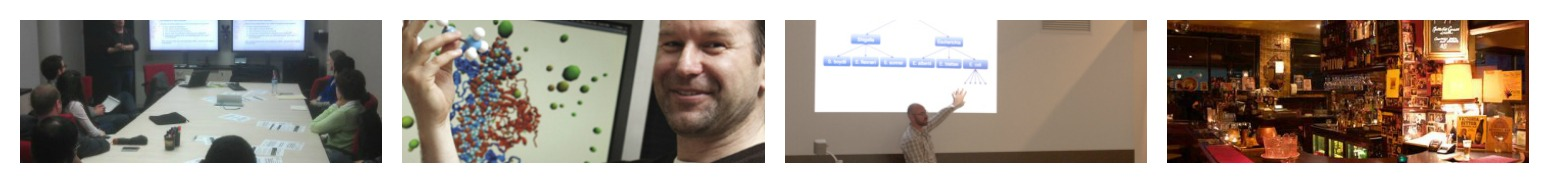
\includegraphics[width=\linewidth]{./images/COMBINE-collage.jpg}
    \vspace{1ex}
    \textbf{Alignment free methods for sequence comparison}\\
    Dr.~Tom Conway, NICTA\\[2ex]
    \textbf{How to get your computer to freeze}\\
    Dr.~Mike Kuiper, VLSCI\\[2ex]
    \textbf{How to give a better research presentation}\\
    Prof. Justin Zobel, The University of Melbourne\\[2ex]
    \textbf{October social event}\\[2ex]
    \textbf{Student Symposium 2012}
\end{frame}

\begin{frame}{Upcoming Events}
    \setlength{\leftmargini}{1.1em}
    \begin{itemize}
        \item Python workshop
        \item \beamerpurple{Student Symposium 2013 (late November)}
    \end{itemize}
    \vspace{1ex}
    Let us know if you would like to present your work!\\[2ex]
    For more information, or if you'd like to volunteer, visit\\
        \beamerpurple{\href{http://www.combine.org.au}{combine.org.au}} or
        \beamerpurple{\href{http://www.facebook.com/combine.australia}{facebook.com/combine.australia}}\\[4ex]
    COMBINE is sponsored by:\quad
    \begin{minipage}[c]{0.2\linewidth}
        \centering
        \href{http://ict4lifesciences.org.au/}{
\includegraphics[height=0.1\paperheight]{./images/ICT-for-Life-Sciences-Forum-logo.png}}
    \end{minipage}\quad
    \begin{minipage}[c]{0.25\linewidth}
        \centering
        \href{http://www.iscbsc.org/}{
\includegraphics[height=0.1\paperheight]{./images/ISCBSC-logo.png}}
    \end{minipage}\\[2ex]
    \textbf{Thank You!}
\end{frame}

\end{document}
